\documentclass{beamer}
\usepackage{tikz}
\newcommand{\should}{\overset{\text{should}}{=}}
\newcommand{\fttheory}[1]{\fcolorbox{blue}{blue}{\color{white}\textbf{#1}\hspace{\textwidth}}}
\newcommand{\ftexampl}[1]{\fcolorbox{orange}{orange}{\color{black}\textbf{#1}\hspace{\textwidth}}}
\newcommand{\ftdata}[1]{\fcolorbox{violet}{violet}{\color{white}\textbf{#1}\hspace{\textwidth}}}
\newcommand{\ftheader}[1]{\fcolorbox{lightgray}{lightgray}{\color{black}\textbf{#1}\hspace{\textwidth}}}
\begin{document}

%-----------------------------------------------------------------------------%
% OVERVIEW
%-----------------------------------------------------------------------------%
\section{Overview}

\begin{frame}{\ftheader{Yield-to-Maturity}}
	\begin{itemize}
		\item In our previous lectures, we saw that market participants borrow/lend at different yields \textit{depending on the term}  
		\item Rather than carry around an entire yield curve whenever we want to recompute the price of a bond, we summarize this information with the \textit{yield-to-maturity} (YTM), with which you are familiar from your previous coursework
		\item Example: consider a 1000 USD, 30-year, 5\% T-bond that makes semi-annual payments, and trades for 1011.9610 USD 
		\item The YTM on this T-bond is the \underline{one} rate that would make the PV of cash-flows equal to the price, namely, 4.9233\%
	\end{itemize}
\end{frame}

\begin{frame}{\ftexampl{YTM Example}}
		Suppose that 1, 2, and 3-year, 100 USD zero-coupon bonds trade for 106.4607, 99.7684, and 93.7438 USD respectively. What should be the YTM of a 3-year, 1000 USD, 10\% coupon bond that makes annual payments? \\
		\pause
	{\color{blue}

		First compute what the price should be.
		\begin{equation*}
			p_{\text{cpn}}\should 1\times106.4607+1\times99.7684+11\times93.7438=1237.4109\text{ USD}
		\end{equation*}
		Then we can compute the YTM using a financial calculator: NPER $=$ 3, PMT $=$ 100 USD, PV $=$ 1237.4109 USD, and FV $=$ 1000 gives us a YTM of 1.7998\%.
	}
\end{frame}

\begin{frame}{Today's Lecture}
	In this lecture, we're going to study how bond prices change in response to changes in YTM using \underline{duration}. We will:
\begin{enumerate}
	\item use duration to compute \%$\Delta$ in price for \%$\Delta$ in YTM;
	\item compute duration of coupon bond;
	\item compute duration of a portfolio of bonds.
\end{enumerate}
\end{frame}

%-----------------------------------------------------------------------------%
% DURATION
%-----------------------------------------------------------------------------%
\section{Duration}

% DURATION--------------------------------------------------------------------%
\begin{frame}{\fttheory{Duration}}
	\textbf{Duration}: The weighted average of the times at each coupon or principal payment is made by the bond. It provides an `weighted average' of the times when you will receive your cash flows. Even though you will receive your bond payments spread over time, duration \underline{one hypothetical point in time} when you will receive your cash-flows.
\end{frame}

% Annuities
\begin{frame}{\fttheory{Treasuries Recap}}
	A $T$-year Treasury makes semi-annual payments.
	\begin{figure}[H]
		\begin{center}
			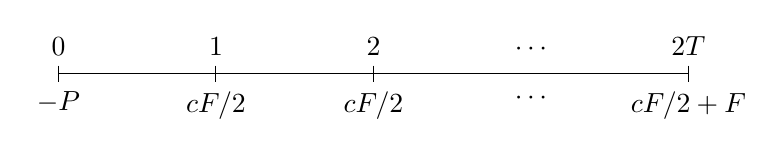
\begin{tikzpicture}
				\draw (0,0) -- (8,0);
				\foreach \x in {0,2,4,8}
				\draw(\x cm,3pt) -- (\x cm, -3pt);
				\draw (0,0) node[above=3pt] {0};
				\draw (2,0) node[above=3pt] {1};
				\draw (4,0) node[above=3pt] {2};
				\draw (8,0) node[above=3pt] {$2T$};
				\draw (0,0) node[below=3pt] {$-P$};
				\draw (2,0) node[below=3pt] {$cF/2$};
				\draw (4,0) node[below=3pt] {$cF/2$};
				\draw (6,0) node[above=3pt, align=center] {$\cdots$};
				\draw (6,0) node[below=3pt, align=center] {$\cdots$};
				\draw (8,0) node[below=3pt] {$cF/2+F$};
			\end{tikzpicture}
		\end{center}
	\end{figure}
where $c\geq0$ is the coupon rate (APR) 
{\scriptsize
\begin{equation*}
	P{\color{red}(y)}\should\frac{cF/2}{(1+y/2)}+\frac{cF/2}{(1+y/2)^2}+\frac{cF/2}{(1+y/2)^3}+\cdots+\frac{cF/2}{(1+y/2)^{2T}}+\frac{F}{(1+y/2)^{2T}}
\end{equation*}
}
where $y$ is the YTM. 
\end{frame}

\begin{frame}{\fttheory{Bond Price Changes}}
Bond price volatility is proportional to the bond's duration; therefore duration becomes a natural measure of interest rate exposure.
\begin{equation*}
	\boxed{\frac{\Delta P}{P}\approx-D\times \frac{y'-y}{(1+y/2)^{2}}}
\end{equation*}
where $y$ is the current YTM (APR), $y'$ is the new YTM (APR) and $D$ is the duration expressed in years. Note that this is for \underline{semi-annual compounding}.
\end{frame}

% DURATION--------------------------------------------------------------------%
\begin{frame}{\fttheory{Duration}}
\begin{center}
    
\includegraphics[scale=.55]{duration}
\end{center}
\end{frame}

\begin{frame}{Duration Problem 1}
Suppose that the duration of a bond is 1.5 years. The YTM is currently 4\% (APR). If the YTM shifts up by 0.5\% in a few days, will there be a gain or a loss? Calculate it.\\
\pause
{\color{blue}
\begin{align*}
	\frac{\Delta P}{P}&\approx-D\times \frac{y'-y}{(1+y/2)^{2}}\\
	&=-1.5\times\frac{0.005}{(1+0.02)^{2}}\times \\
	&=-0.7209\%
\end{align*}
}
\end{frame}

% DURATION--------------------------------------------------------------------%
\begin{frame}{\fttheory{Computing Duration}}
\begin{itemize}
	\item We compute the duration in two steps. 
	\item Compute \textit{weights}:
	{\scriptsize
	\begin{align*}
		w_{1}{\color{red}(y)}&=\frac{F/P}{(1+y/2)},\: w_{2}{\color{red}(y)}=\frac{F/P}{(1+y/2)^2},\:w_{3}{\color{red}(y)}=\frac{F/P}{(1+y/2)^3}\\
		&\hspace{.5in},\ldots,w_{2T}{\color{red}(y)}=\frac{F/P}{(1+y/2)^{2T}}
	\end{align*}
	}
	\item The duration is  
	{\scriptsize
	\begin{align*}
		D{\color{red}(y)}&\should\frac{1}{2}\times (c/2)w_{1}{\color{red}(y)}+1\times(c/2)w_{2}{\color{red}(y)}+\frac{3}{2}\times (c/2)w_{3}{\color{red}(y)}\\
		&\hspace{.5in}+\cdots+\frac{2T}{2}\times (c/2)w_{2T}{\color{red}(y)}+\frac{2T}{2}\times w_{2T}{\color{red}(y)}
	\end{align*}
	}
	\item For the interested, 
	{\scriptsize
	\begin{equation*}
		D{\color{red}(y)}=-\frac{P'(y)}{P(y)}(1+y/2)
	\end{equation*}
	}
\end{itemize}
\end{frame}


\begin{frame}{\ftexampl{Duration Problem 1}}
	Compute the duration of a 2-year, 100 USD, 8\% coupon T-note with a YTM of 5\%.
	\pause
	{\small \color{blue}
	The price of this bond is 105.6430 USD, so $F/P=$0.9466
	\begin{align*}
		w_{1}&=-\text{PV}(\text{NPER}=1,\text{I/Y}=2.5,\text{PMT}=0.,\text{FV}=0.9466)=0.9235\\
		w_{2}&=-\text{PV}(\text{NPER}=2,\ldots)=0.9010\\
		w_{3}&=-\text{PV}(\text{NPER}=3,\ldots)=0.8790\\
		w_{4}&=-\text{PV}(\text{NPER}=4,\ldots)=0.8576
	\end{align*}
	and hence
	\begin{align*}
		D &= 0.5\times(4\%\times w_{1})+1.0\times(4\%\times w_{2})+1.5\times(4\%\times w_{3})\\
		&\hspace{.5in}+2.0\times(4\%\times w_{4})+2.0\times w_{4}\\
	&=1.8911\text{ years}
	\end{align*}
	}
\end{frame}

\begin{frame}{\ftexampl{Duration Problem 2}}
	Compute the duration of a 10-year, 100 USD, zero coupon bond with a YTM of 5\% (compound semi-annually).\\
	\pause
	{\small \color{blue}
	The price of this bond is 61.0271 USD, so $F/P$=1.6386
	\begin{align*}
		w_{1}&=0\\
		\vdots\\
		w_{19}&=0\\
		w_{20}&=-\text{PV}(\text{NPER}=20,\text{I/Y}=2.5,\text{PMT}=0.,\text{FV}=1.6386)=1
	\end{align*}
	\begin{align*}
		D&=10\text{ years}
	\end{align*}
	Intuitive! 
	}
\end{frame}

\begin{frame}{\fttheory{Duration of a Portfolio}}
\begin{itemize}
	\item The duration of a portfolio is the portfolio of the duration, meaning:
	\begin{equation*}
	D_{P}=\frac{V_{1}}{V}D_{1}+\frac{V_{2}}{V}D_{2}+\dots +\frac{V_{M}}{V}D_{M}
	\end{equation*}
	where $V_{i}$ is the value of the security $i$, $V$ is the total value of the portfolio, and $D_i$ is the duration of security $i$.
	\item \textbf{Important:} In the above formula, $V_i$ is positive for an asset, and $V_i$ is negative for a liability. Also remember that 
	\begin{equation*}
	V=V_1+V_2+\dots + V_M
	\end{equation*}
\end{itemize}
\end{frame}

\begin{frame}{\ftexampl{Duration of a Portfolio Problem 1}}
An investor has 100k USD to invest. She borrows another 80k by issuing 10-year zero coupon bonds worth 80k today. She invests 70k in 3-year zero coupon bonds and 110k in a coupon bond with duration of 4 years. What is the duration of her portfolio?\\ 
\pause 
{ \color{blue} The total value of her portfolio is 100k USD ($=$110k$+$70k$-$80k).  
\begin{equation*} 
D_p=\frac{70}{100}\times 3 +\frac{110}{100}\times 4 -\frac{80}{100}\times 10=-1.5 \text{ years}
\end{equation*} 
}
\end{frame} 

\begin{frame}{\ftexampl{Duration of a Portfolio Problem 2}}
A credit union lends Bonnie 500k USD to buy a house. The loan is a vanilla 15-year fixed with a duration of 6 years. Clyde deposits 400k USD in a 15-year deposit account with a duration of 10 years. The credit union has 100k USD in retained earnings that it invests in a 10-year zero-coupon bond. What is the duration of the bank's portfolio?
\pause 
{ \color{blue} The total value of the credit union's portfolio is 200k USD ($=$500k+100k$-$400k).  
\begin{equation*} 
	D_p=\frac{500}{200}\times 6 +\frac{100}{200}\times 10 -\frac{400}{200}\times 10=0\text{ years}
\end{equation*} 
A banker's dream come true!
}
\end{frame} 

\section{Heterogeneity}

% DURATION AND THE COUPON RATE------------------------------------------------%
\begin{frame}{\fttheory{Duration Heterogeneity}}
    \begin{itemize}
        \item Holding the term constant, a bond’s duration is higher when the coupon rate is lower;
        \item Holding the coupon rate constant, a bond’s duration generally increases with its term 
    \end{itemize}
\end{frame}

% DURATION AND THE COUPON RATE------------------------------------------------%
\begin{frame}{\fttheory{Duration and the Coupon Rate}}
    \begin{center}
        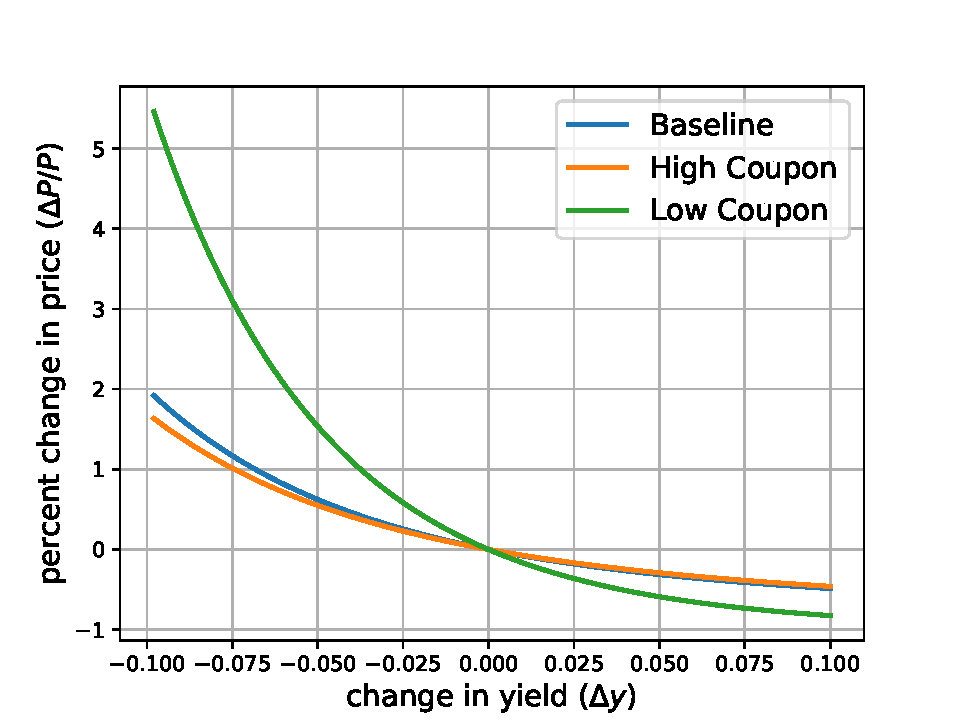
\includegraphics[scale=.55]{coupon}
    \end{center}
\end{frame}

% DURATION AND TERM-----------------------------------------------------------%
\begin{frame}{\fttheory{Duration and Term}}
    \begin{center}
        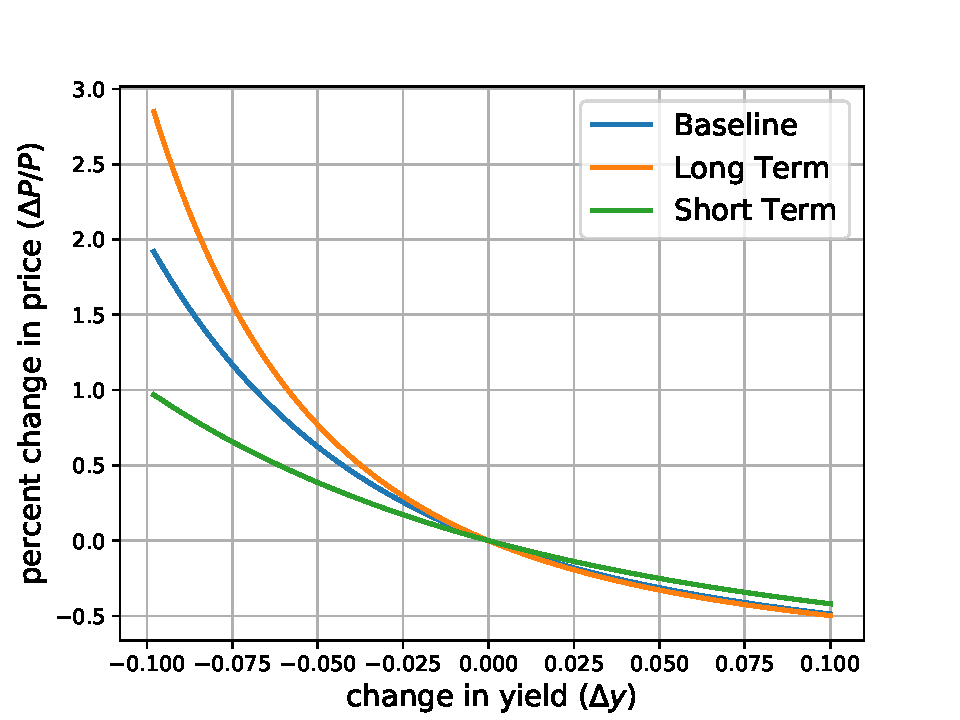
\includegraphics[scale=.55]{term}
    \end{center}
\end{frame}

% IMMUNIZATION----------------------------------------------------------------%
\section{Immunization}
\begin{frame}{\fttheory{Immunization}}
    \begin{itemize}
        \item Banks and financial institutions have a natural mismatch between the asset side and the liability side 
        \item Immunization refers to strategies used by investors to shield their overall financial position from exposure to interest rate fluctuations.
        \item If this is not taken into consideration, a change in interest rates could run havoc with the institution’s balance sheet, threatening bankruptcy
		\item The goal is to find a portfolio (or balance sheet) with a duration of zero
    \end{itemize}
\end{frame}

\begin{frame}{\ftexampl{Immuzation of Portfolio Problem}}
Suppose a bank manager has a one-time liability of 100k USD due in 5-years. How much of a 10-year zero-coupon bond can she buy to immunize her portfolio?
{ \color{blue} Her portfolio is worth $X-$100k USD. 
\begin{equation*} 
	0=D_p=\frac{X}{X-100}\times 10-\frac{100}{X-100}\times 5
\end{equation*} 
Multiply both sides by $X-100$ and solve for $X$:
\begin{equation*}
	0=10X-500\:\Rightarrow\:X=50\text{k USD}
\end{equation*}
}
\end{frame} 

\end{document}
